% main.tex
\documentclass[conference]{IEEEtran}

% ---- Packages ----
\usepackage{graphicx}
\usepackage{amsmath,amssymb}
\usepackage[hidelinks]{hyperref}
\usepackage{siunitx}
\usepackage{booktabs}
\usepackage[dvipsnames]{xcolor}

% TikZ
\usepackage{tikz}
\usetikzlibrary{arrows.meta,positioning,shapes.geometric,shapes.misc,shapes.symbols,fit}

% Safer node styles (avoid using 'step' as a key)
\tikzset{
  block/.style   = {draw, rounded corners, minimum width=2.6cm, minimum height=8mm, align=center},
  small/.style   = {draw, minimum width=2.0cm, minimum height=7mm, align=center},
  store/.style   = {draw, rectangle, minimum width=2.2cm, minimum height=10mm, align=center, fill=gray!10},
  flowstep/.style= {draw, rectangle, minimum width=2.8cm, minimum height=9mm, align=center},
  line/.style    = {-{Latex[length=2mm]}}
}

% Allow slightly tighter floats but keep abstract first
\setlength{\textfloatsep}{10pt plus 2pt minus 2pt}

% ---- Title ----
\title{AITL on Space: A Robust Three-Layer Architecture\\
with a Tri-NVM Hierarchy (SRAM / MRAM / FRAM)\\
for Long-Duration Spacecraft Autonomy}

\author{
\IEEEauthorblockN{Shinichi Samizo}
\IEEEauthorblockA{Independent Semiconductor Researcher\\
Former Engineer at Seiko Epson Corporation\\
Email: \href{mailto:shin3t72@gmail.com}{shin3t72@gmail.com}\quad
GitHub: \url{https://github.com/Samizo-AITL}}
}

\begin{document}
\maketitle

% -------- Abstract must come before any floats --------
\begin{abstract}
We propose \emph{AITL on Space}, a three-layer control architecture
(Robust Core, FSM Supervisor, AI Adaptor) implemented on a \SI{22}{nm}
FDSOI SoC with a hardened tri-NVM hierarchy (SRAM/MRAM/FRAM).
The system targets ultra-robust autonomy under radiation, thermal cycling,
and long-term drift. This paper outlines the architecture, an 11D
state-space plant model (8--20D extensible), an \mbox{$H_\infty$}
mixed-sensitivity design flow, and a verification pipeline from
FPGA HIL to ASIC.
\end{abstract}

\section{Introduction}
Long-duration missions require high availability under TID/SEE
and thermal cycles. Conventional PID+Flash architectures face
reliability limits. We motivate AITL on Space.

\section{System Architecture}
AITL comprises: (i) Robust Core (for $H_\infty$/MPC/SMC),
(ii) FSM Supervisor (Safe/Nominal/Recovery, FDI/FDI\!I),
and (iii) AI Adaptor for long-term re-identification.
A tri-NVM hierarchy---SRAM for execution, MRAM for logs/code
(ECC+scrub, A/B slots), and FRAM for safe boot---ensures persistence.

% ---- Fig.1 AFTER abstract (here, in Section II) ----
\begin{figure}[!t]
  \centering
  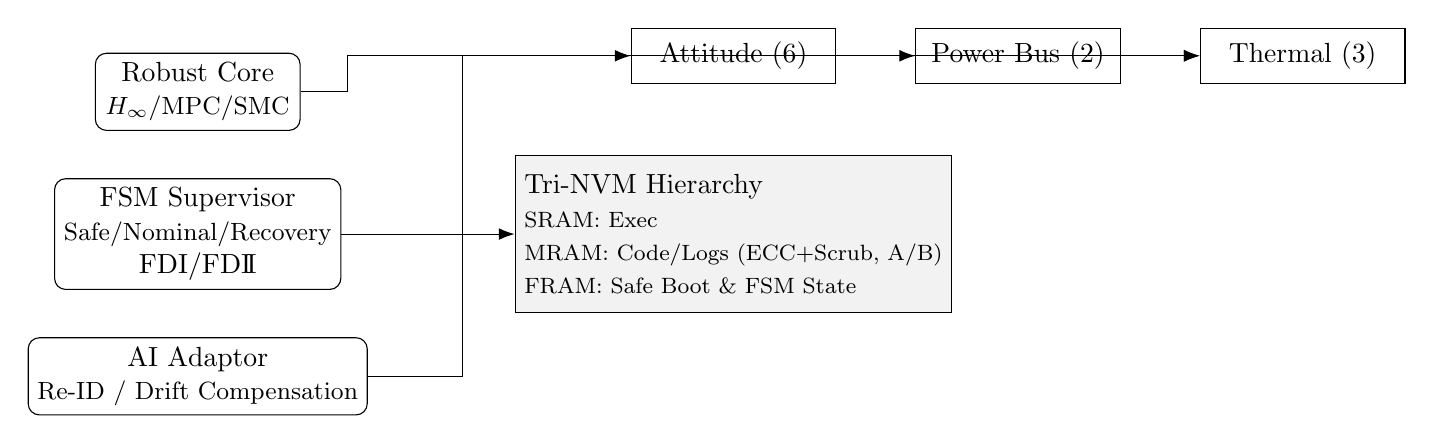
\begin{tikzpicture}[node distance=6mm]
    % Left stack
    \node[block] (core) {Robust Core\\ \small $H_\infty$/MPC/SMC};
    \node[block, below=of core] (fsm) {FSM Supervisor\\ \small Safe/Nominal/Recovery\\ FDI/FDI\!I};
    \node[block, below=of fsm] (ai)  {AI Adaptor\\ \small Re-ID / Drift Compensation};

    % Plant and buses
    \node[store, right=22mm of fsm, minimum width=3.5cm, minimum height=2.0cm, align=left] (tri) {Tri-NVM Hierarchy\\
      \footnotesize SRAM: Exec\\
      \footnotesize MRAM: Code/Logs (ECC{+}Scrub, A/B)\\
      \footnotesize FRAM: Safe Boot \& FSM State};

    \node[small, above=9mm of tri, minimum width=2.6cm] (att) {Attitude (6)};
    \node[small, right=10mm of att, minimum width=2.6cm] (pwr) {Power Bus (2)};
    \node[small, right=10mm of pwr, minimum width=2.6cm] (thm) {Thermal (3)};

    % Connections
    \draw[line] (core.east) -- ++(6mm,0) |- (att.west);
    \draw[line] (fsm.east)  -- (tri.west);
    \draw[line] (ai.east)   -- ++(12mm,0) |- (thm.west);

    \draw[line] (att.east) -- (pwr.west);
    \draw[line] (pwr.east) -- (thm.west);
  \end{tikzpicture}
  \caption{AITL on Space architecture with Robust Core, Supervisor FSM, AI Adaptor, and the tri-NVM hierarchy.}
  \label{fig:arch}
\end{figure}

\section{Mathematical Model}
We use an 11D plant that couples attitude (6), power bus (2),
and thermal nodes (3). The discrete-time model is
\begin{align}
  x_{k+1} &= A x_k + B u_k + E w_k, \\
  y_k     &= C x_k + D u_k + v_k. \label{eq:ss}
\end{align}
Extensions scale to 20D with translational axes and bias states.

% ---- Fig.2 (control block) ----
\begin{figure}[!t]
  \centering
  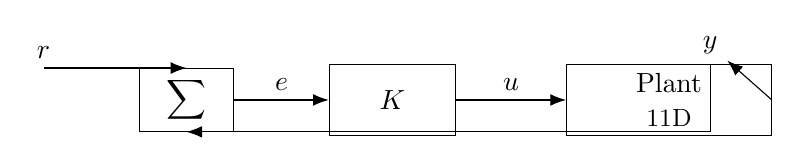
\begin{tikzpicture}[node distance=9mm]
    \node[small, minimum width=1.2cm] (sum) {$\displaystyle\sum$};
    \node[flowstep, right=12mm of sum, minimum width=1.6cm] (K) {$K$};
    \node[flowstep, right=14mm of K, minimum width=2.6cm] (plant) {Plant\\ \small 11D};
    \node[above left=0mm and 10mm of sum] (r) {$r$};
    \node[above right=0mm and -10mm of plant] (y) {$y$};

    \draw[line] (r) |- (sum.north);
    \draw[line] (sum.east) -- (K.west) node[midway, above] {$e$};
    \draw[line] (K.east) -- node[midway, above] {$u$} (plant.west);
    \draw[line] (plant.east) -- (y);
    \draw[line] (y) |- (sum.south);
  \end{tikzpicture}
  \caption{Closed-loop schematic used for $H_\infty$ synthesis on the 11D plant.}
  \label{fig:loop}
\end{figure}

\section{$H_\infty$ Mixed-Sensitivity Design}
Weights $(W_1,W_2,W_3)$ shape sensitivity, effort, and complementary
sensitivity. \emph{EduController} exports JSON plant/weights; AITL-H
synthesizes output-feedback $K$ and fixed-point realization.

\section{Verification Pipeline}
FPGA HIL injects SEU bursts and sensor outages; metrics include
safe-mode time ($<\! \SI{1}{s}$), recovery rate ($\ge \! \SI{99}{\%}$),
and ECC statistics. Physical design proceeds to 22FDX tape-out; FEM
closes thermal/packaging effects.

% ---- Fig.3 (verification flow) ----
\begin{figure}[!t]
  \centering
  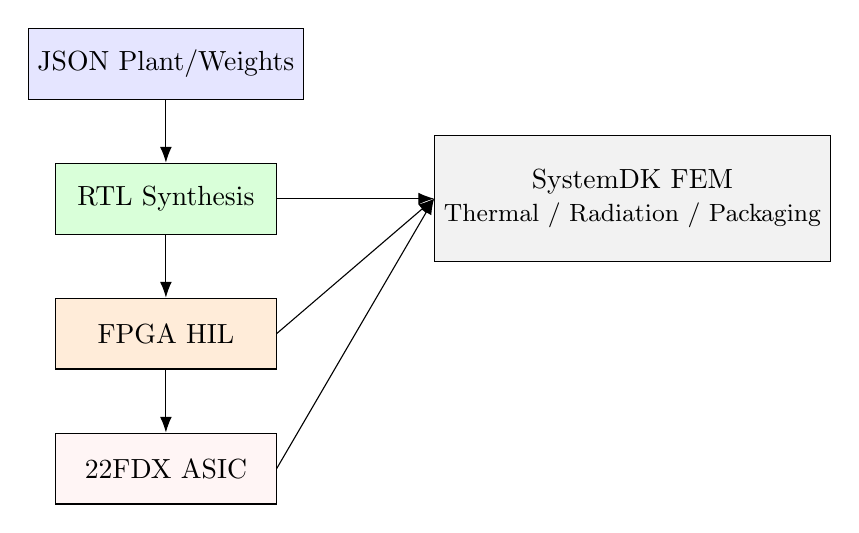
\begin{tikzpicture}[node distance=8mm]
    \node[flowstep, fill=blue!10]   (json) {JSON Plant/Weights};
    \node[flowstep, below=of json, fill=green!15] (rtl)  {RTL Synthesis};
    \node[flowstep, below=of rtl,  fill=orange!15] (hil)  {FPGA HIL};
    \node[flowstep, below=of hil,  fill=pink!15]   (asic) {22FDX ASIC};

    \node[store, right=20mm of rtl, minimum width=3.5cm, minimum height=1.6cm, align=center] (fem)
      {SystemDK FEM\\ \small Thermal / Radiation / Packaging};

    \draw[line] (json) -- (rtl);
    \draw[line] (rtl)  -- (hil);
    \draw[line] (hil)  -- (asic);
    \draw[line] (rtl.east) -- (fem.west);
    \draw[line] (hil.east) -- (fem.west);
    \draw[line] (asic.east) -- (fem.west);
  \end{tikzpicture}
  \caption{Verification pipeline from JSON design to RTL, FPGA HIL, and ASIC; FEM closes the loop with thermal and radiation scenarios.}
  \label{fig:pipeline}
\end{figure}

\section{Conclusion}
AITL on Space offers a practical path to resilient autonomy
for deep-space missions.

\section*{References}
\begin{thebibliography}{99}
\bibitem{doyle} G.~Doyle, \emph{Feedback Control Theory}.
\bibitem{colinge} J.-P.~Colinge, \emph{Silicon-on-Insulator Technology}.
\end{thebibliography}

\section*{Author Biography}
\noindent
\textbf{Shinichi Samizo} received the M.S.\ degree in Electrical
and Electronic Engineering from Shinshu University, Japan.
He worked at Seiko Epson Corporation as an engineer in semiconductor
memory and mixed-signal device development, and contributed to inkjet
MEMS actuators and PrecisionCore printhead technology. He is currently
an independent semiconductor researcher focusing on process/device
education, memory architecture, and AI system integration.
Contact: \href{mailto:shin3t72@gmail.com}{shin3t72@gmail.com}.

\end{document}
